%KECReportFormat.tex
%%%%%%%%%%%%%%%%%%%%%%%%%%%%%%%%%%%%%%%%%%%%%%%%%%%%%%%%%%%%%%%%%%%%%%%%%%%
%DO NOT MAKE CHANGES IN THIS FILE

\documentclass[12pt, a4paper]{report}
\usepackage[left = 1.5in, right = 1in, top = 1in, bottom = 1in]{geometry}%for margin
\usepackage{amsfonts, amsmath, amssymb} %for mathematical equations
\usepackage{graphicx} %for images
\usepackage{times} %font Times New Roman Font
\usepackage{float} %required if you use H(strictly here) position for floats
\usepackage[skip = 8pt,tableposition=top, figureposition=bottom]{caption}%adjust spacing of captions and specify where captions are
\usepackage{hyperref} % for easy Navigation in document, also puts links in TOC, LOF, LOT...
\usepackage{setspace} %to change line spacing in some portion \singlespacing \onehalfspacing \doublespacing
\usepackage{acro} %for List of Abbrreviation and Symbol
\acsetup{first-style = short} % set to display only short form on the command \ac{}

%packages required for complex tables
\usepackage{bigstrut} 
\usepackage{multirow}

\renewcommand{\contentsname}{Table of Contents} %Change TOC Heading ... default is "Contents" 

\parindent 0pt	%removes the indent in paragraph
\setlength{\parskip}{18pt}	%for paragraph spacing
\renewcommand{\baselinestretch}{1.5}   %Line Spacing = 1.5 line-spaces

%to reduce spacing in sections
\usepackage{titlesec}
\titlespacing*{\section}{0pt}{0pt}{0pt} %left, top, bottom spacings
\titlespacing*{\subsection}{0pt}{0pt}{0pt}
\titlespacing*{\subsubsection}{0pt}{0pt}{0pt}
\titlespacing*{\paragraph}{0pt}{0pt}{0pt}
\titlespacing*{\subparagraph}{0pt}{0pt}{0pt}

%adjust fontsizes\ of sections
\titleformat*{\section}{\fontsize{14pt}{18pt}\bfseries}
\titleformat*{\subsection}{\fontsize{13pt}{18pt}\bfseries}
\titleformat*{\subsubsection}{\fontsize{12pt}{18pt}\bfseries}
\titleformat*{\paragraph}{\fontsize{12pt}{18pt}\bfseries}
\titleformat*{\subparagraph}{\fontsize{12pt}{18pt}\bfseries}

%to reduce separation between points in list
\usepackage{enumitem}
\setlist[enumerate]{nosep} % no separation between items in enumerate
\setlist[itemize]{nosep} % no separation between items in itemize
%use \vspace{-18pt} before list to reduce paragraph spacing between list and preceeding paragraph.

%Changes for Chapter Heading Spacing and formats for numbered chapters
\makeatletter
\def\@makechapterhead#1{%
  %\vspace*{50pt}%
  {  \MakeUppercase{\ifnum \c@secnumdepth >\m@ne
        \fontsize{16pt}{1}\bfseries \@chapapp \space \thechapter\vspace{5pt}\\
    \fi
    \interlinepenalty\@M
     \bfseries #1}\par\nobreak
    %\vskip 0pt
  }}
\makeatother

%%%%%%%%%%%%%%%%%%%%%%%%%%%%%%%%%%%%%%%%%%%%%%%%%%%%%%%%%%%
%to adjust Heading spacings and fonts For unnumbered chapters, TOC, LOF ...
\makeatletter
% Redefine the \chapter* header macro to remove vertical space
\def\@makeschapterhead#1{%
  %\vspace*{50\p@}% Remove the vertical space
  {\newpage \parindent \z@ \raggedright
    \normalfont
    \interlinepenalty\@M
    \center \fontsize{16pt}{1} \bfseries \MakeUppercase{#1}\par\nobreak
    %\vskip 18\p@ % adjust space after heading 18pt
  }}
\makeatother 
%%%%%%%%%%%%%%%%%%%%%%%%%%%%%%%%%%%%%%%%%%%%%%%%%%%%%%%%%%%

%%%%%%%%%%%%%%%%%%%%%%%%%%%%%%%%%%%%%%%%%%%%%%%%%%%%%%%%%%%%%%%%%%%%%%%%%%%
% newcommand for generating Cover Page
\newcommand{\KECcoverpage}
{
\begin{titlepage}
\begin{center}
\Large{\textbf{KANTIPUR ENGINEERING COLLEGE}}\\
\large{\textbf{(Affiliated to Tribhuvan University)}}\\
\large{\textbf{Dhapakhel, Lalitpur}}\\
\vfill	%vertically fill the space 
\begin{figure}[h] % h: put logo "here"
\begin{center}

\includegraphics[width=25mm, height = 25mm]{images/logo.png}
\end{center}
\end{figure}

\large{\textbf{[Subject Code: \subCode]}}\\ %Change This Line
\large{\textbf{A \MakeUppercase{\project} \MakeUppercase{\doc} ON}}\\ %Change This Line
\Large{\textbf{\MakeUppercase{\projectTitle}}}\\

\vfill	%vertically fill the space 
\large{\textbf{Submitted by:}}\\
\large{\textbf{\submittedBy}}\\
\vfill	%vertically fill the space 
\textbf{A \MakeUppercase{\project} SUBMITTED IN PARTIAL FULFILLMENT OF THE REQUIREMENT FOR THE DEGREE OF \MakeUppercase{\degree}}\\

\vfill	%vertically fill the space 
\large{\textbf{Submitted to:}}\\
\large{\textbf{\submittedTo}}\\
\vfill
\large{\textbf{\defMonth, \defYear}}
\pagebreak
\end{center}
\end{titlepage}
}
%%%%%%%%%%%%%%%%%%%%%%%%%%%%%%%%%%%%%%%%%%%%%%%%%%%%%%%%%%%%%%%%%%%%%%%
% newcommand for generating Cover Page
%Title Page
\newcommand{\KECtitlepage}
{
\begin{titlepage}
\begin{center}
\Large{\textbf{\MakeUppercase{\projectTitle}}}\\

\vfill	%vertically fill the space 

\large{\textbf{Submitted by:}}\\
\large{\textbf{\submittedBy}}\\

\if{\ne{\supervisor}{none}} \\ Displays Supervisor name only if it is not "none"
	\vfill	%vertically fill the space 
	\large{\textbf{Supervised by:}}\\
	\large{\textbf{\supervisor}}\\
	\large{\textbf{\degSup}}\\
\fi
\vfill	%vertically fill the space 
\textbf{A \MakeUppercase{\project} SUBMITTED IN PARTIAL FULFILLMENT OF THE REQUIREMENT FOR THE DEGREE OF \MakeUppercase{\degree}}\\

\vfill	%vertically fill the space 
\large{\textbf{Submitted to:}}\\
\large{\textbf{\submittedTo}}\\
\large{\textbf{Kantipur Engineering College}}\\
\large{\textbf{Dhapakhel, Lalitpur}}\\

\vfill
\large{\textbf{\defMonth, \defYear}}
\thispagestyle{empty}\\ %to remove page number
\pagebreak
\end{center}
\end{titlepage}
}
%%%%%%%%%%%%%%%%%%%%%%%%%%%%%%%%%%%%%%%%%%%%%%%%%%%%%%%%%%%%%%%%%%%%%%
%command for copyright page
\newcommand{\KECcopyright}
{
\chapter*{Copyright}%Required only for Final Defense of Major Project
\addcontentsline{toc}{chapter}{Copyright}
The author has agreed that the library, Kantipur Engineering Collage, may make this report freely available for inspection. Moreover the author has agreed that permission for extensive copying of this report for scholarly purpose may be granted by the supervisor(s), who supervised the project work recorded herein or, in their absence, by the Head of the Department wherein this project was done. It is understood that due recognition will be given to the author of this report and to the \submittedTo, Kantipur Engineering College in any use of the material of this report. Copying or publication or other use of this report for financial gain without approval of the \submittedTo, Kantipur Engineering College and author’s written permission is prohibited.\par Request for permission to copy or to make any other use of the material in this report in whole or in part should be addressed to:

Head\\
\submittedTo\\
Kantipur Engineering College\\
Dhapakhel, Lalitpur\\
Nepal
}
%%%%%%%%%%%%%%%%%%%%%%%%%%%%%%%%%%%%%%%%%%%%%%%%%%%%%%%%%%%%%%%%%%%%%%
%command for Approval Letter
\newcommand{\KECapproval}
{
\chapter*{Kantipur Engineering College
\vskip -10pt}%Required only for Final Defense of Major Project
\begin{center}
\fontsize{12.8pt}{1} %size decreaced to adjust department name in single line
\textbf{
\MakeUppercase{\submittedTo}\\ %for department name
}
\vskip 10pt
\fontsize{16pt}{1}
\textbf{APPROVAL LETTER}
\end{center}
\vskip -16pt
\addcontentsline{toc}{chapter}{Approval Letter}%
The undersigned certify that they have read and recommended to the Institute of Engineering for acceptance, a project report entitled "\projectTitle " submitted by \\
\submittedBy \\
in partial fulfillment for the degree of \degree. \par
{\vspace{25pt}
..........................................\\
Supervisor\\
\supervisor \\
\degSup\\
\vspace{25pt}\\
..........................................\\
External Examiner\\
\external\\
\degExternal\\
\vspace{25pt}\\
..........................................\\
\hod\\
Head of Department\\
\submittedTo
\vspace{10pt}\\
Date: \defMonth\space\defDay ,\space \defYear
\singlespacing\par
} %single spacing for the texts inside {}
}

%command for list of abbreviations
\newcommand{\KECloa}
{
\chapter*{List of Abbreviations}
\addcontentsline{toc}{chapter}{List of Abbreviations}
\vskip -42pt % to reduce space due to invisivle acronym class name
{
\singlespacing
\printacronyms[include=abbr, name= ]
}

}

%command for list of symbols
\newcommand{\KEClos}
{
\chapter*{List of Symbols}
\addcontentsline{toc}{chapter}{List of Symbols}
\vskip -42pt % to reduce space due to invisivle acronym class name{
{
\singlespacing
\printacronyms[include
=symbol, name= ]
}
}

%command to adjust toc, lof, lot spacing
\newcommand{\KECadjusttocspacings}
{
\parskip 0pt % to remove paragraph spacing in TOC, LOF ...
\renewcommand{\baselinestretch}{0.1} % to adjust line spacing in toc
\newcommand*{\noaddvspace}{\renewcommand*{\addvspace}[1]{}}
\addtocontents{lof}{\protect\noaddvspace} %remove extra vertical space in LOF
\addtocontents{lot}{\protect\noaddvspace} %remove extra vertical space in LOT
} %includes the file KecReportFormat.tex that include all necessary formatting
%%%%%%%%%%%%%%%%%%%%%%%%%%%%%%%%%%%%%%%%%%%%%%%%%%%%%%%%%%%%%%%%%%%%%%%%%%%
%Define Macros for Details of your Project
\newcommand{\project}{Major Project} %Specify "Major Project" or "Minor Project"
\newcommand{\projectTitle}{End-To-End Encryption Chatapp } %specify "Title" of Your Project
\newcommand{\doc}{Report} % specify the document you are preparing eg. "Proposal", "Mid-Term Report" or "Final Report" 
% Note that You have to submit "Final Report" for Pre-final defense as well.
\newcommand{\subCode}{CT755} %specify Subject of Your Project
\newcommand{\degree}{Bachelor in Computer Engineering} %specify your degree
\newcommand{\submittedBy}%Specify Names and Roll/Symbol Numbers of the Project Group Members
{
%Edit Member Names and Roll/Symbol No. and adjust width (\makebox[width]) if necessary 
\makebox[7cm]{Anup chaudhary \hfill [KAN075BCT009]}\\
\makebox[7cm]{Chris Gurung \hfill [KAN075BCT023]}\\
\makebox[7cm]{Himalaya Pal \hfill [KAN075BCT029]}\\
\makebox[7cm]{Kundan Giri \hfill [KAN075BCT030]}
%\makebox[9cm]{Member Name \hfill [Roll/Symbol No.]}\\
} % Note that You must write your "Symbol Numbers"(Exam Roll Numbers) for Final Defenses

\newcommand{\submittedTo}{Department of Computer and Electronics Engineering} %specify your department
\newcommand{\hod}{Er. Rabindra Khati} %specify Head ot the department
\newcommand{\defYear}{2023} %Defense Year
\newcommand{\defMonth}{March} %Defense Month- January, February, ...
\newcommand{\defDay}{29} %specify Defense Day- 1, 2, ...

\newcommand{\supervisor}{none} % Specify Name of Supervisor for Major Project (write "none" if no Supervisor is assigned)
\newcommand{\degSup}{Supervisor's Designation\\Second Line of Designation (if required)} %Specify Designation of Supervisor for Major Project, use multiple lines (\\) if necessary
\newcommand{\external}{External's Name} %Specify Name of External for Major Project (Required for Black Book)
\newcommand{\degExternal}{External's Designation\\Second Line of Designation (if required)} %Specify Name of External for Major Project (Required for Black Book) , use multiple lines (\\) if necessary
%%%%%%%%%%%%%%%%%%%%%%%%%%%%%%%%%%%%%%%%%%%%%%%%%%%%%%%%%%%%%%%%%%%%%%%%%%%

%%%%%%%%%%%%%%%%%%%%%%%%%%%%%%%%%%%%%%%%%%%%%%%%%%%%%%%%%%%%%%%%%%%%%%%%%%%
%Define Abberviations and Symbols
% NOTE that Only those Abberviations and Symbols that are included in document(using command \ac{}) will be displayed in the List of Abberviations and Symbols.

%class 'abbr': for List of Abbreviations
\DeclareAcronym{HTML}{ 
  short = HTML ,
  long  = Hypertext Markup Language ,
  tag = abbr
}% declares acronym named "UN". Use \ac{UN} for short and \acl{UN} for long form. 

\DeclareAcronym{CSS}{
  short = CSS ,
  long  = Cascading Style Sheet ,
  tag = abbr
}


%%%%%%%%%%%%%%%%%%%%%%%%%%%%%%%%%%%%%%%%%%%%%%%%%%%%%%%%%%%%%%%%%
% class `symbol': for List of Symbols
\DeclareAcronym{transparencyFactor}{
  short = \ensuremath{\alpha} ,
  long  = Transparency Factor ,
  sort  = Transparency Factor , % string to compare for sorting symbols... default string is the acronym name -"transparencyFactor"
  tag = symbol
}% declares acronym named "transparencyFactor". Use \ac{UN} for short and \acl{UN} for long form.

\DeclareAcronym{areaOfTriangle}{
  short = \ensuremath{a} , % use \ensuremath{a} instead of $a$
  long  = Area of Triangle ,
  sort  = Area of Triangle , % string to compare for sorting symbols
  tag = symbol
}
%%%%%%%%%%%%%%%%%%%%%%%%%%%%%%%%%%%%%%%%%%%%%%%%%%%%%%%%%%%%%%%%%%%%%%%%%%%%%%%%%%%%%%%%%%%%%%%%%%%%

%%%%%%%%%%%%%%%%%%%%%%%%%%%%%%%%%%%%%%%%%%%%%%%%%%%%%%%%%%%%%%%%%%%%%%%%%%
%The Document
\begin{document}
\KECcoverpage % command defined in KECReportFormat
\KECtitlepage % command defined in KECReportFormat

\pagenumbering{roman} % starts pagenumberins in Roman numerals i, ii, ...

%Copyright Page is required for FINAL REPORT only. Comment this section for other Reports.
\KECcopyright
% defined in KECReportFormat.tex
\KECapproval

%Approval Page is required for FINAL(Black Book Binded) REPORT of MAJOR PROJECT only. Comment this section for other Reports. 
% defined in KECReportFormat.tex

\chapter*{Abstract} % The summary of your report
\addcontentsline{toc}{chapter}{Abstract}%to include this chapter in TOC 
Data security is a crucial concern that ought to be managed to help protect vital data. Cryptography is one of the
conventional approaches for securing data and is generally considered a fundamental data security component that
provides privacy, integrity, confidentiality, and authentication.

In the current world where communication has been made easy such that you could talk to a person on the other side of the world with a press of the button. With the increase in availability of internet service you can send texts, photos ,files through the internet in a matter of seconds and for far less cheaper. This is achieved through different chat applications. With the increased usage of such chat applications the contents of such messages contains more that just simple messages to friends and families but also very important information and files which on the wrong hands could cause a huge catastrophe. As such End-to-End security is needed to safely exchange private information with each other without worrying about data. With this project we aim to provide an End-to-End encrypted chat apps.

This project approach End-to-End encryption method to provide  secure communication that prevents third parties from accessing data while it's transferred from one end system or device to another.
The End-to-End encryption method is implemented using the Asymmetric key encryption algorithm (RSA). We used RSA to encrypt that encoded data.
In this way we can maintain the data more securely.


\par
\textbf{\textit{Keywords$-$}} RSA

\chapter*{Acknowledgment}
\addcontentsline{toc}{chapter}{Acknowledgment}%to include this chapter in TOC
We would like to acknowledge Er. Bikash Shrestha, our project supervisor who is providing us guidence and
helping us with different views of application, development and scalability as well as helped us in development of our project.
His guidence has been corner stone in developing chat app. We are able to accomplish this project with his valuable direction and suggestions.\par
We would like to express our notable thanks to Department of Computer and Electronics Engineering
for providing us environment to dig the latest technology, investigate it and do research on those areas as Major project.
We are also grateful to Er. Rabindra Khati, HOD, Department of Computer and Electronics Engineering
for presenting useful suggestions regarding the queries put forward regarding the project.\par
Our special appreciation goes to Lecturers of Kantipur Engineering College for guiding us in this project
and helping to better cope with the difficulties along with giving supportive hands. Without their
valuable guidence it would have been difficult for us to come to a conclusion to work with this technology.\par
Last but not least, we would appreciate all our seniors and friends for their support and constant inspiration which helped us to
withstand in our success in this project.
%to display members name under Acknowledgement
\begin{flushright}
	\vskip -20pt
	\setstretch{1.2}
	\submittedBy
\end{flushright}



%to adjust spacings for TOC, LOF, LOT
{
%%%%%%%%%%%%%%%%%%%%%%%%%%%%%%%%%%%%%%%%%%%%%%%%%%%%%%%%%%%%%%%%%%%%%%%%%%%
%TOC, LOF and LOT
\KECadjusttocspacings % defined in KECReportFormat.tex to adjust spacings
\makeatletter
% to add vskip of 18 point which is reduced when parskip is set to 0 in \LECadjustspacings
\def\@makeschapterhead#1{%
	%\vspace*{50\p@}% Remove the vertical space
	{\newpage \parindent \z@ \raggedright
			\normalfont
			\interlinepenalty\@M
			\center \fontsize{16pt}{1} \bfseries \MakeUppercase{#1}\par\nobreak
			\vskip 18\p@ % adjust space after heading 18pt
		}}
\makeatother

\tableofcontents % prints table of contents
\listoffigures % prints list of figures
\addcontentsline{toc}{chapter}{List of Figures}
%\listoftables % prints list of table
%\addcontentsline{toc}{chapter}{List of Tables}
}
%%%%%%%%%%%%%%%%%%%%%%%%%%%%%%%%%%%%%%%%%%%%%%%%%%%%%%%%%%%%%%%%%%%%%%%%%%%

%comment this chapter if you don't have List of Abbreviations
%\KECloa % defined in KECReportFormat
%comment this chapter if you don't have List of Symbols
%\KECl1os % defined in KECReportFormat

\newpage
\pagenumbering{arabic} % starts pagenumbering in arabic numerals

\chapter{Introduction}
\section{Background}\label{sec:bkgrnd}%label your section if you require to refer them somewhere else in your document.
Digital communications surveillance is a major
security concern in the world at large. End-to-End (E2E)
encryption in mobile communication applications delivers
confidentiality between users, defending messages against
snooping. Several widespread communication tools
(WhatsApp, Signal, Telegram, iMessage) have implemented
end-to-end encryption, as a major selling point. Yet, the
understand of the security goals (confidentiality, integrity,
authentication) remain vague to users, such as how the
security goals offer protection, and if they value that
protection.\par
With the growing use of the internet as a medium for
communication, it becomes imperative to secure personal
and business’ online communications. Consequently, the
motivation to execute attacks increases and preventing
against these attacks using technology that is almost
unbreakable was considered. This technology, if employed
accurately, could avert large-scale attacks. End-To-End
Encryption suggests a maintainable answer to the continuing
challenges of internet security . End-to-end encryption
describes the process of secure exchange of data from
sender to recipient; preventing third-parties from accessing
the data during transmission. All information is encrypted by
the sender and the recipient decrypts it. During
transmission, the content is completely encrypted, which
means that no third parties can access or tamper with it
during transmission . Several cryptographic algorithms
are used alone or combined for the encryption purposes.\par
The components of End-To-End Encryption includes :
The identity component authenticates users. The protocols
component handles the key exchange and the algorithm. The
algorithm uses scientific process to encrypt the data, and it
cannot be decrypted without the predetermined key. Secure
implementation and operation ensure the End-To-End
Encryption process is not vulnerable to attacks on the
hardware side. These components work together to deliver a
system that operates efficiently to offer the best security to
end users.\par
Internet security is an extremely vital issue in computer
science, due to the increasing acceptance of online
communication. Since e-mailing services became public,
questions arose about how secure they are. Furthermore, the
need to secure the internet was made popular by shopping,
banking, and other financial transactions via the internet .
Is End-To-End Encryption the best technology to ensuring
data security? In recent times, most of the communications
between clients and servers are secured using Transport
Layer Security. However, communications between clients
are not yet secured . With plaintext communication
vulnerable to hackers . Consequently, security
researchers have proffered the usage of End-To-End
Encryption.\par
This research focused on providing a performance
evaluation experiment on RSA algorithm and its usage in end to end encrypted
chat app. RSA is based
on number theory, using two prime numbers or
mathematical operation to randomly produce the public and
private keys. The public key (which is public) is used for
encryption, and the private key (which is private) is used for
decryption. Sender encrypts the communication using public
key of the recipient and when the communication is
received, the recipient can decrypt it with its private key.\cite{paley}


\pagebreak
\section{Problem statement}
\vspace{-18pt}
Traditional messaging like SMS are very unsecure as it travels through the network in plain text. Since messages might contain very sensitive informations the messages shouldn't be accessible to any other person beside the actual people involved in the conversation. Furthermore in unsecure messaging any third party can pretend to be the intended person and gain access or send wrong information.


\section{Objectives}
The application aims to provide data security in communication system. The application focuses on
simplicity of design, having user-friendly interface and to be easily understood. \\
The main objectives of the application can be enumerated as follows:
\vspace{-18pt}
\begin{itemize}
	\item To provide end-to-end text message security.
	\item To provide platform for sending messages from one person to another.
\end{itemize}

\section{Applications}
The application is an online web application. This system can be used to provide end to end encryption of data and also used to provide secure connection between user between users with smooth and clean UI.

\section{Project features}
The application, is targeted towards the general population, so the core features of this applications can be listed below:

\vspace{-18pt}
\begin{itemize}
	\item We can send messages
	\item It provides end-to-end data security in communication system.
	\item Simple and ease for general population
\end{itemize}

\section{Feasibility Analysis}
Feasibility is a measure of how benificial or practical the development of a system will be to an organization or enterprise.
In other words, a feasibility study is an evaluation and analysis of the potential of the proposed project which is based on extensive investigation and reasearch to give
full comfort to the decision masker. A system should have a responsible cost and should be technically and operationally feasible to be actually implemented.
The two criteria to judge feasibilty are cost required and value to be attained. The feasibility of "End to End encryption Chatapp " is analyzed under the following four headings:

\subsection{Economic Feasibility}
Economic Feasibility is the measure of the cost effectiveness of the project or the solution. This is often called a cost benifit analysis. \par
Based on our economic analysis for development and operational cost,
the system is being developed and operated economically. For development,
the required devices are readily available, so it is feasible. Also,
it is economically feasible to the consumers as it costs no charge to use the platform.

\subsection{Schedule Feasibility}
Based on the objectives and the time left for the development.
The schedule is found to be feasible.

\subsection{Technical Feasibility}
Technical Feasibility is the measure of the practically of a specific technical solution and the availability of technical resources and expertise.\par
Technically, the system is feasible enough and easy-to-use
for both technical and non-technical groups of people. It provides
a user-friendly environment along with features using the latest technologies.
The system provides a layout most of the applications people are used to anyway
so it will be easy to use.

\subsection{Operational Feasibility}
Operational feasibility is the measure of how a well specific solution will work in the organization.
It is also measure of how people feel about the system of the project. It also analyze the inside operation on how a deemed process
will work, be implemented, and dealing with changes resistance and acceptance.\par
For the operation of the system, the person does
not need to excel in using a computer. Since, the event
may not always be related to the technical fields, someone
with minimum knowledge about computer and technology can also get
benefit from the system. Similarly, one can get access to the system
as a web-based application. There is no requirement of huge and expensive hardware.

\section{System Requirements}

\subsection{Software Requirement}
Application is targeted towards a general market,
so it is aimed to be fully optimized enough for any low-range to
high-range systems, so listed below are
the software requirements for the development and operation of this system:
\vspace{-18pt}
\begin{itemize}
	\item Operating System: Windows 8 or above
	\item Browsers: Google Chrome, Firefox, etc
	\item Mongodb, Node.js Server
	\item React js
\end{itemize}

\subsection{Hardware Requirement}
Hardware configuration and requirements for the
operation of this application are as follows:
\vspace{-18pt}
\begin{itemize}
	\item Intel Core 2 Duo Processor (Recommended i-series processors or more) with minimum of 2GB RAM for application operation
	\item Server with optimum node speed
\end{itemize}
%\subsection{Referring Section}
%This is an example of referring Section \ref{sec:bkgrnd} of page \pageref{sec:bkgrnd}. \\



\chapter{Literature Review}

\section{Research on End-to-End Encryption chat app}
There are currently millions of monthly active users worldwide of different chat applications currently. There are two types of architecture in those applications, client-server and peer-to-peer networks. In a peer-to-peer network, there is no central server and each user has his/her own data storage. On the contrary, there are dedicated servers and clients in a client-server network and the data is stored on a central server. Security and privacy in chat applications have a paramount importance but few people take it seriously. In a test done by the Electronic Frontier Foundation, most of the popular messaging applications failed to meet most security standards. These applications might be using the conversations as an information for certain purposes. Moreover, reading the private conversations is certainly unacceptable in terms of privacy.  Most applications only used Transport Layer Security (TLS) for securing channel, the service provider has full access to every message exchanged through their infrastructure . Therefore, these messages can be accessed by attackers. Therefore to maintain protection and privacy, messages should be encrypted from sender to receiver and no one can read messages even the service provider, in addition to protecting the local storage of the device.\\
There are different Encryption algorithms that can  be utilized  to  provide secure  messaging environment. Thus, messages will circulate as  encrypted form in transmission medium, not as clear text. Somebody who has seized encrypted data does not obtain original message from the encrypted  data  unless they  possess  the  necessary  method or  a  key.  Encryption  methods  are divided into the following categories: private key cryptography and public key cryptography.\\
In a symmetric key algorithm, the sender and receiver must have a shared key set up in advance and keep secret from all other parties; the sender uses this key for encryption, and the receiver uses  the  same  key  for  decryption.  In  this  case,  except  for  transmitted  encrypted  message, encryption  key  must  also  be  submitted  confidentially,  which  is  one  of  the  disadvantages of private-key cryptography.
If a third person who has managed to enter the system operator or listen to transmission medium
seizes the  key value,  s/he can turn  the  encrypted data into  original data.  The most  important feature of public key cryptography which is another method is that the key value used to encrypt the message is different from the key value used to decrypt the message. Each user has two keys
in this method: public key and private key. The public key of the user can be viewed by anyone.
The private key is kept secret by the user. When someone wants to send a message to user, they
use the user's public key and create the encrypted message and then send the encrypted data to
user. The user  decrypts the  encrypted data with  her/his private  key  and obtains  a meaningful
message.\cite{Sabah2017}\\
\section{Research on Client / Server Cryptography-Based Secure Messaging
  System Using RSA Algorithm }
In today’s world, computer networking has become an
integral part of life. There are many different networks
available to share information between groups of devices
through a shared communication medium . They are
mainly differentiated by the physical medium and protocol
standards. Ethernet is a prime wired networking standard
which is an obvious choice for many network applications
due to reliability, efficiency, and speed. Ethernet standard is
used in various application segments . Figure below
shows the Client/Server model architecture that has been
used in most network systems and in this study specially.
\begin{figure}[H]
	\centering
	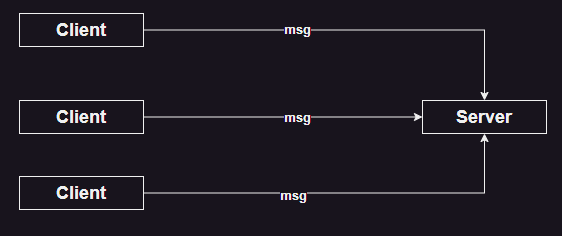
\includegraphics[width=160mm]{images/clientserver.png}
	\caption{A CLient/Server architecture}
	\label{figclientserver} % for referencing
\end{figure}

The client side could be any type of smart devices
(desktop, laptop, smart phone, etc.). The server part is one
device that control and pass messages and opining the
connections among clients and/or between clients and server
. The Internet part could be one device to isolate the
network overall into two main parts: client(s) and server, it
could be a switch or hub or router or just a cable.\\
A very important aspect in the world of software
development is the security of data that flows through open
communication channels. In our web applications,
there is an intensive exchange of data via different
protocols, like http, between client applications which
presented as browser applications and
server side applications. The importance and confidentiality
of data may be different depending on the specifics of the
web application, and the possibility of interception by a third
party increases with perfection of hacking techniques in the
world of IT. What can be done to prevent access to the
data by your traffic listener? If we exchange with data
between the client applications and server we don’t want the
information to be stored as open text on the server, which will
be accessible in case of server crack.\\
Every day people used chat area, through the users
(clients) scan chat or send messages to selected users.
However, the security components in chat area application
are to make sure all information from clients is protected
from hackers. The chat messages from users can easily
transform by expert hackers, without a good enough security
components. In this way, a chat area interface (CAI) is
required technique to secure a chat message from hackers.
The cryptography is significant to keep private data secure
and to avoid unauthorized access.\\
Basically, the proposed messaging/chat system is
expected to provide a communication channel between
clients via a server using encryption based on RSA in a
Client/Server environment. The goal for this study is
to use client/server architecture to accomplish secure chat
between clients. All the used encryption
processes based on RSA algorithm.\\
The very term client-server was initially applied to the
software architecture, which described the distribution of the
execution process by the principle of interaction of two
software processes, one of which in this model was called the
client and the other the server. The client process requested
some services, and the server process ensured their execution.
It was assumed that one server process can serve a lot of
client processes. One of the client/server application is that
“chatting”. Chatting alludes to one kind of correspondence
over the Internet that offers a continuous transmission of
instant messages from sender to beneficiary or over a server
that is control and deal with the gatherings (customers) to
convey.\cite{sonmez2017development}\\
\subsection{Client/Server}
The used client/server model describes how
a server provides resources and services to one or
more clients. Examples of servers including web servers, chat
servers, and file servers. Each of these servers provide
resources to client devices. Most servers have a one-to-many
relationship with clients, meaning a single server can provide
resources to m Computers. In order to meet the main
requirements of businesses, networks themselves are
becoming quite complex multiple clients at one time .\cite{sonmez2017development}\\

\subsection{Chat Service}
A secure chat service provides the ability to have real time
secure discussions among users electronically, one-to-one or
in groups session . A public network accumulates
information slightly, rather than on a user’s individual
computer that is used to keep in touch with people.\cite{sonmez2017development} A secure
chatting between client and server to make a safe and reliable
communication, the benefits are :
\vspace{-18pt}
\begin{itemize}
	\item Allows for instant communications between users
	\item Uses real time chat over the network that can
	      eliminate costly long distance charges.
	\item Allows for rapid query and rapid responses.
\end{itemize}
While the negative points of chat service can be listed as
following:
\vspace{-18pt}
\begin{itemize}
	\item Security problems of instant messaging program
	\item Secure chats in most cases are routed through a
	      server system, where the service is provided and that is a
	      single point where all messages can be intercepted.
	\item Chat programs can provide an open avenue of
	      attack for hackers, crackers, spies and thieves.
\end{itemize}

\subsection{RSA Encryption}
In this, an encrypted chat program designed to
ensure a safe mode of communication between two users. It
uses RSA encryption to encode and decode messages in a
terminal window. RSA is widely used public-key
cryptograph and authentication system for data encryption of
digital messaging transactions such as e-mail over the
intranet, extranet and Internet. Clients exchange public keys
and encrypt outgoing text with the intended recipient’s public
key. Each user connects to a central server which
forwards messages to the intended recipient. On the receiving
end, the program utilizes a client’s private key to decrypt
received messages. In 1977, Ron Rivest, Adi Shamir and
Leonard Adleman introduced a cryptographic algorithm,
RSA, which is named for the first letter in each of its
inventors’ last name. RSA’s motivation is DiffieHellman Algorithm which describes the idea of such an
algorithm that enables public-key cryptosystem.\\
Encryption algorithm is deployed to encrypt messages
exchanged with the proposed chat gateway. The chat messaging
environment showed a great potential to host realtime
interactive interaction system which is supported by RSA
encryption methodology to preserve the security of the
message stream. \\
Choosing the key size in RSA encryption is of great
importance. As the size of the key increases, the security level
of the system, the complexity and the resistance of encrypted
text increases . These advantages make it difficult to
decrypt ciphertexts and break passwords. However, in
addition to these advantages, the encryption key creation
time, text encryption time, and mobile device RAM
consumption increase . These disadvantages are
factors that will influence the effective use of the application.
For this reason, the advantages and disadvantages of key
dimensions should be determined and the most suitable key
size should be preferred. \cite{sonmez2017development}\\
Currently, RSA is secure using 2048 and 4096-bit key lengths.
Larger keys will be required in a near future.Theoretically, RSA keys that are 2048 bits long should be good until 2030. If so, isn't it a bit early to start using the 4096-bit keys that have become increasingly available in encryption-enabled applications?
According to " NIST Special Publication 800-57 Part1"2048-bit RSA keys are roughly equivalent to a Security Strength of 112. Security strength is simply a number associated with the amount of work required to break a cryptographic algorithm. Basically, the higher that number, the greater the amount of work required.
It implies longer keys are more difficult to break and are hence more secure.\\

\begin{tabular}{ |p{3cm}||p{3cm}|  }

	\hline
	Security Strength & RSA Key length \\
	\hline
	$<=80 $           & 1024           \\
	112               & 2048           \\
	128               & 3072           \\
	192               & 7680           \\
	256               & 15360          \\
	\hline
\end{tabular}
\\
According to that publication, 112 security strength (which corresponds to 2048-bit keys) is considered to be acceptable until 2030. Again, here's a portion of that table for reference.\\

\begin{tabular}{ |p{3cm}||p{3cm}|p{3cm}|  }

	\hline
	Security Strength & Through 2030 & 2030 and beyond \\
	\hline
	$<112 $           & Disallowed   & Disallowed      \\
	112               & Acceptable   & Disallowed      \\
	128               & Acceptable   & Acceptable      \\
	192               & Acceptable   & Acceptable      \\
	256               & Acceptable   & Acceptable      \\
	\hline
\end{tabular}
\\
\\
So now we know 2048 bit keys are indeed acceptable until 2030 as per NIST.
So where does that put our 4096 bit keys? Incidentally, the document is
silent about this particular key length. However, because the two tables
indicate that 3072-bit keys (whose security strength is 128) and 7680-bit
keys (whose security strength is 192) are good beyond 2030, we can safely
say 4096 bit keys (which are somewhere in between)
should likewise be considered secure enough then.\\
In fact, since 2048-bit keys are supposed to be disallowed after 2030, we
know for certain that 4096 bit keys are going to be more suitable in
production environments than 2048 keys when that time comes. But since
we're still at least a decade away from 2030, it's probably not yet
necessary to migrate from 2048 to 4096, right?
So why then are we already seeing options for 4096-bit keys in some security applications?\\
Well, there is  couple of reasons. One is simply to make the application
future proof. A future proof security solution can mitigate the risk of
cyber threats. We know that cyber criminals are always one step ahead of
security professionals, so we're not 100percent sure 2048-bit keys are going to
remain unbreakable before 2030. (Source: NIST Special Publication 800-57 Part1)

In RSA, a sender encrypts a message using the recipient's public key, and
the recipient decrypts the message using their private key.
sWhen transferring an RSA public key, it is important to ensure that the
key cannot be easily intercepted and replaced by an attacker. One common
technique for protecting the key during transfer
is to use salting, also known as padding or randomization.

Salting involves adding random data to the beginning or end of the
public key before transferring it. This random data, or salt, makes
it more difficult for an attacker to intercept and replace the key
with their own. The recipient of the key can then strip off the salt
before using the key for encryption or decryption.

In summary, salting is a simple and effective technique for protecting
RSA public keys during transfer. It adds an extra layer of security to
the key exchange process and makes it more difficult for attackers to
intercept and replace the key.


\section{Existing system:}
In this section we briefly introduce many of the popular chat applications. Some of these applications are not public or open source so it is difficult for these to get evaluated by the developer’s community, security experts or research academic.

\subsection{Viber}
Viber is an instant messaging and Voice over IP (VoIP) application for
smartphones developed by Viber Media. In addition to instant messaging,
users can exchange images,
video and audio media messages. Viber recently supported the end-to-end
encryption to their service, but only for one-to-one and group conversations
in which all
participants are using the latest Viber version 6.0 for Android, iOS or
Windows 10. At this time, in the Viber iOS application for iPhone and iPad,
attachments such as images and videos which are sent via the iOS Share
Extension does not support end-to-end encryption.
Viber has privacy issues such as adding a friend without his knowledge
or adding him to a group without his permission. Plus that, local storage
is not secured. It is not
open source making it difficult to evaluation.\cite{Sabah2017}

\subsection{Whatsapp}
WhatsApp is one of the most popular messaging application, recently
enabled end-to-end encryption for its 1 billion users across all platforms.
WhatsApp uses part of a security protocol developed by Open Whisper System,
so provides a security-verification code that can share with a contact to
ensure
that the conversation is encrypted. It is difficult to trust in
WhatsApp application completely because the application is not open source,
making it difficult to verify the functioning process and match them
with the work of the encryption protocol which was announced. .\cite{Sabah2017}

\subsection{Telegram}
Telegram is an open source instant messaging service enables users
to send messages, photos, videos, stickers and files. Telegram provides
two modes of messaging
is regular chat and secret chat. Regular chat is client-server based on
cloud-based messaging, it does not provide end-to-end encryption, stores
all messages on its
servers and synchronizes with all user devices. More, local storage is
not encrypted by default. Secret chat is client-client provides end-to-end
encryption. Contrary to regular chat messages, messages that are sent in a
secret chat can only be accessed on the device that has been initiated a
secret chat and the device that has been accepted a secret chat they
cannot be accessed on other devices. Messages sent within secret chats
can be deleted.
at any time and can optionally self-destruct. Telegram uses its
own cryptographic protocol MTProto which is based on 256-bit symmetric
AES encryption, 2048-bit RSA encryption, and Diffie–Hellman secure key
exchange, and has been criticized by a significant part of the cryptographic
community about its security. The registration process of Telegram, Viber
and WhatsApp depend on SMS. SMS is transported via Signaling System 7 (SS7)
protocol. The vulnerability lies in SS7. Attackers exploited SS7 protocol
to login into
victim's account by intercepting SMS messages. Because of Telegram cloud-based,
the attacker exploits it and makes full control of the victim account and can
prevent him to enter into his account. To make the account more secure should
activate two-factor authentication \cite{Sabah2017}

\subsection{Facebook Messenger}
Facebook Messenger is a popular messaging service
available for Android and iOS. It provides two modes of
messaging one is regular chat and another is secret conversations.
Regular chat does not provide end-to-end encryption only
secure communication by using TLS,  and it stores all
messages on its servers. Secret conversations have  the
same idea of Telegram secret chat . \cite{Sabah2017}

\section{The Challenge- Making it real-time}
For any app to feel real-time, the user needs to be kept updated with any activity happening as soon as possible. The challenge arises in selecting and implementing a suitable development technique. With the traditional request-response model, we have few options:
\subsection{Refresh Webpage}
The user might refresh the web page time-to-time to check for message updates. But that is not an optimal solution. This may result in bad UX.

\subsection{HTTP Protocol}
The concept of HTTP request-response is widely used. But this requires establishing a TCP connection every time data is sent to the server. Being a one-way synchronous communication protocol, this may result in a lot of overheads while creating and destroying a TCP connection every time a message is sent in real-time chat applications.
\begin{figure}[H]
	\centering
	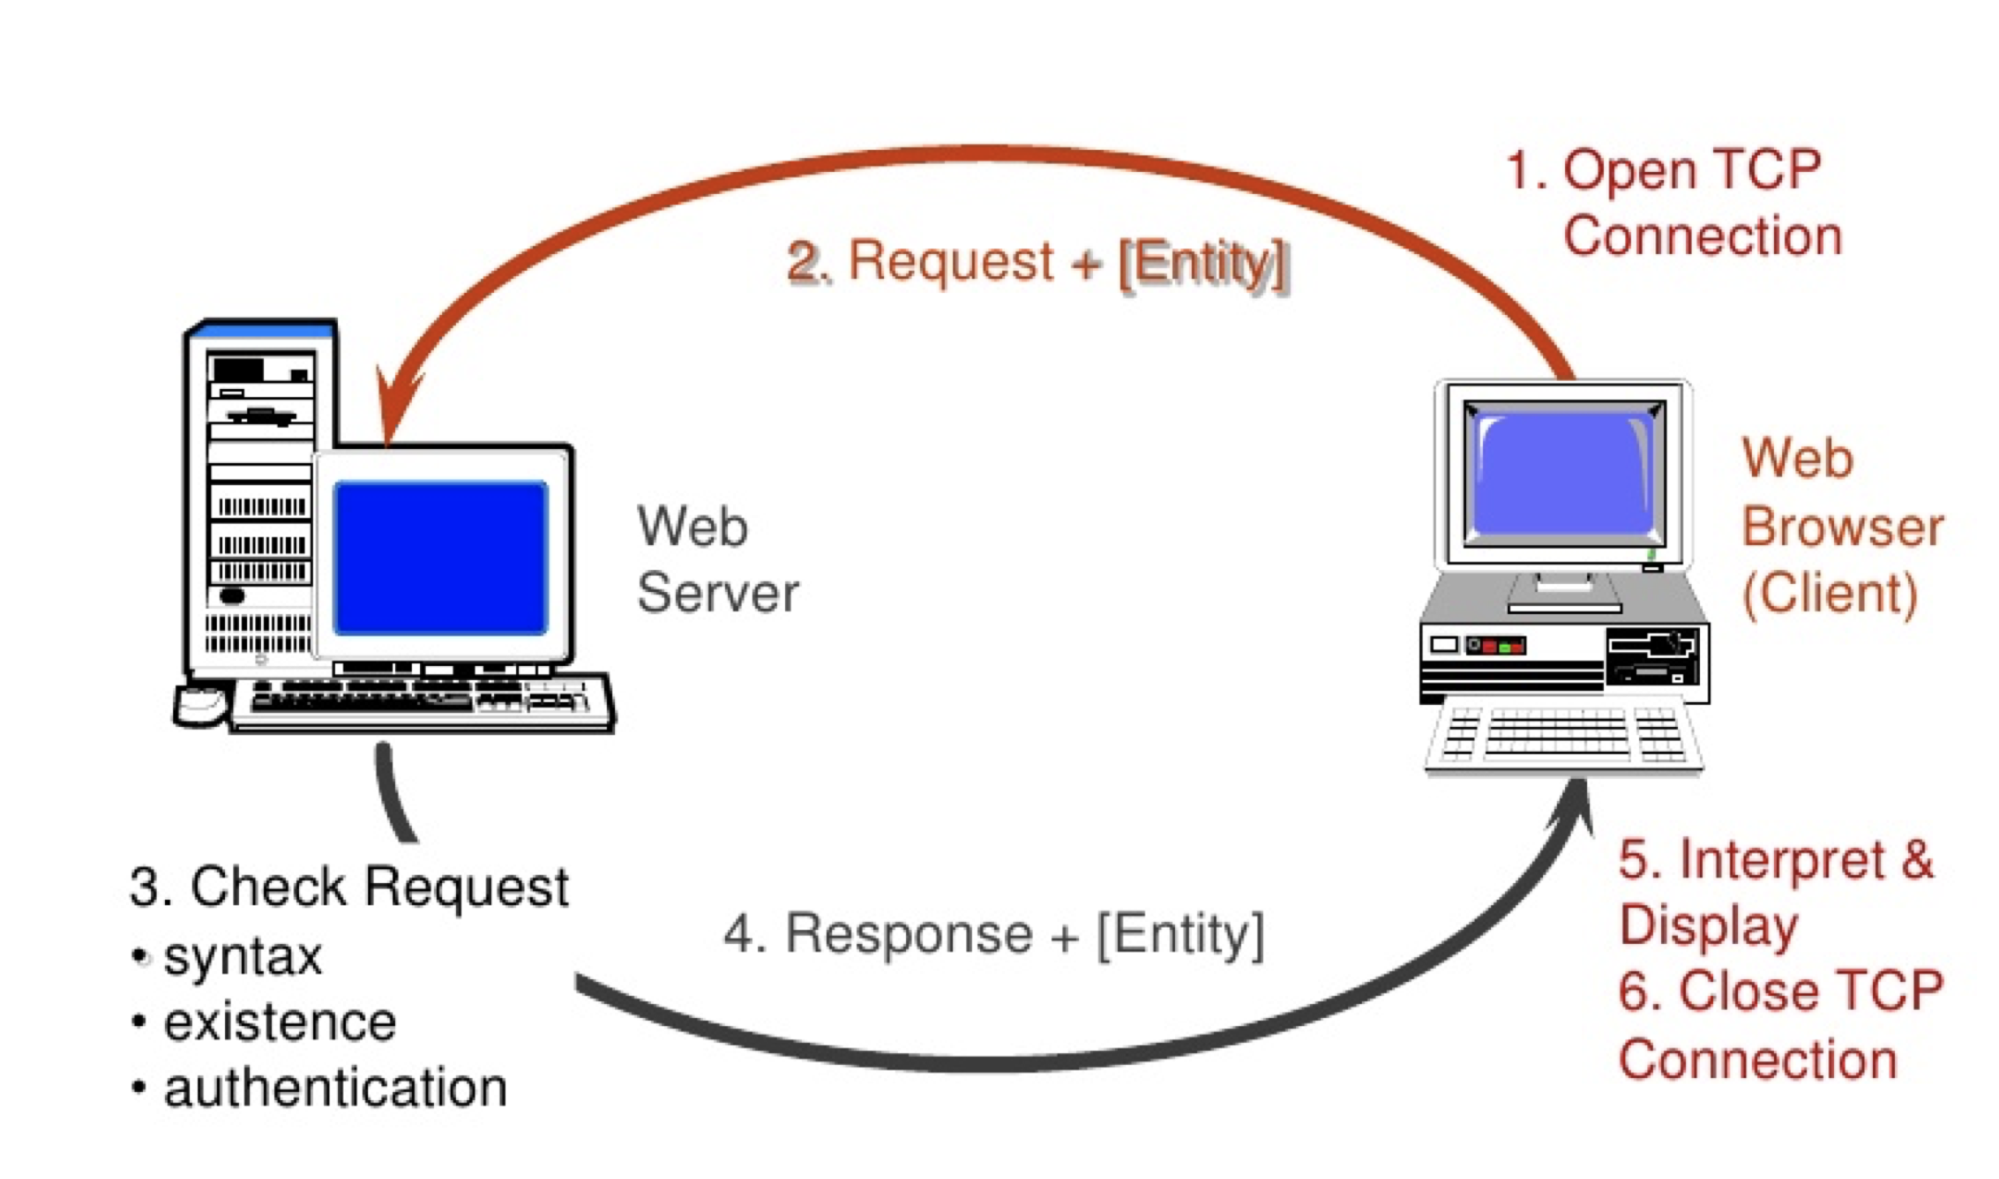
\includegraphics[width=140mm, height=160mm]{images/Http_request-response_cycle.png}
	\caption{Http Request-Response Cycle} %figure name
	\label{figusecase} % for referencing
\end{figure}



\section{Web Sockets}
This concept resolves most of the issues we just discussed. It implements instant two-way communication of messages with a persistent connection just as required for developing a real-time system. NodeJS offers several libraries to implement this technology. What we will be utilizing for our application is the Web Socket API with ‘Socket.io’ library.
\subsection{Socket.io Api}
Socket.IO is a library that enables low-latency, bidirectional and event-based communication between a client and a server. It is built on top of the WebSocket protocol and provides additional guarantees like fallback to HTTP long-polling or automatic reconnection.

\subsection{Socket.io Handshake}
The handshake in Socket.IO is like any other information technology related handshake. It is the process of negotiation, which in Socket. IO's case, decides whether a client may connect, and if not, denies the connection.

\subsection{Exchanging Messages}
\vspace{-18pt}
\begin{itemize}
	\item The messages are exchanged in the form of data frames rather than a stream of data
	\item It is a bi-directional flow of data
	\item The event listeners of the ws object are used for message exchange
	\item The closing handshake can take place either by the client or the server. Reconnection has to be done manually.
\end{itemize}

\chapter{Methodology}

\section{Required Algorithm:}

\subsection{Overview of RSA Algorithm}
RSA encryption algorithm, which is based on the idea of ensuring the secure transfer of data in the digital environment and the algorithmic difficulty of separating the integer factorization, is a type of public-key encryption method. Nowadays, it is also known as both the most commonly used encryption method and the method that allows digital signatures. It was created by Ron Rivest, Adi Shamir and Leonard Adleman  in 1978. Prime numbers are used for key generation process in RSA encryption method.This makes it possible to create a safer structure. How the encryption and decryption processes
are done with RSA algorithm is shown in below figure,
\begin{figure}[H]
	\centering
	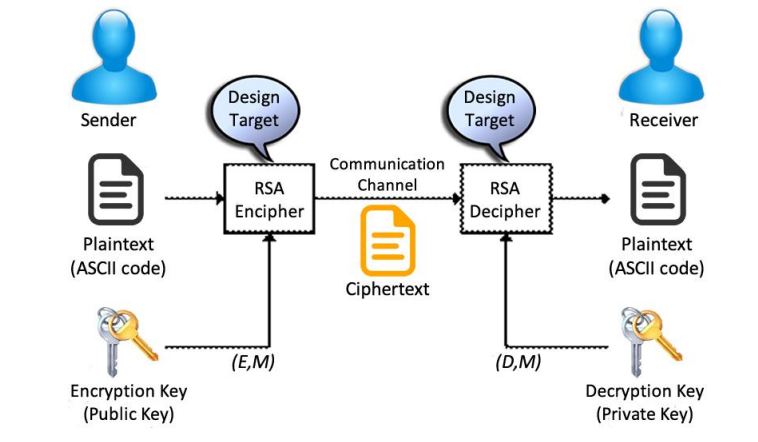
\includegraphics[width=160mm]{images/rsa algo.png}
	\caption{RSA algorithm working mechanism}
	\label{figdecisionalgo1} % for referencing
\end{figure}
\pagebreak

\subsection{RSA algorithm structure}
\subsubsection{Steps:}
\vspace{-18pt}
\begin{itemize}
	\item Choose two very large random prime integers: p and q
	\item Calculate n = p*q and z = (p-1)(q-1)
	\item Choose a number e as public key where 1 $<$ e $<$ z which is co-prime with z
	\item Calculate d = e-1mod(p-1)(q-1)
	\item You can bundle private key pair as (n,d)
	\item You can bundle public key pair as (n,e)
\end{itemize}
After creating public and private keys, information which must be sent is encrypted with the
public key.
\subsubsection{Encryption and decryption processes are done as follows:}
\vspace{-18pt}
\begin{itemize}
	\item The cypher text C is found by the equation where M is the original
	      message
	\item The message M can be found from the cypher text C by the equation M = C$^d$ mod n
	\item A text encrypted with the public key can only be solved with the private key
\end{itemize}
\subsection*{Salting}
Salting is the process of adding random data to a password or other sensitive information before it is hashed.
The salt is a random string of characters that is unique to each user and is added to the password before it is hashed.
The purpose of salting is to make it much more difficult for attackers to use precomputed hash tables to reverse-engineer
a password from its hash value. Without the salt, an attacker could use a precomputed hash table to compare a list of hashed
passwords to a database of stolen password hashes and quickly find matches, allowing them to gain unauthorized access to user accounts.
However, with a unique salt for each password, the precomputed hash tables become useless, as the attacker would need to generate a new hash table for each salt used.
In summary, salting is an important security measure that helps to protect user passwords and other sensitive information by making
them more resistant to attacks by malicious actors.
\subsection*{Hashing}
Hashing is a process of converting input data of any length into a fixed-size output, called a hash or message digest.
The hash function takes the input data and applies a one-way mathematical algorithm to it to produce a unique hash value.
Hashing is used in many applications such as password storage, data integrity verification, and digital signatures.
Hashing and RSA are two separate cryptographic concepts that are often used together in digital signatures. RSA is a public key encryption algorithm,
while hashing is a one-way function used to create a unique fixed-size output (hash) from an input of any size.When we say that hashing is a one-way function,
it means that it is easy to compute the hash value from the input data, but it is computationally infeasible to recover the original input data from the hash value.
This property of hashing is important for ensuring the integrity and security of data. For example, in password storage, instead of storing the actual password, the password is hashed and the hash value is stored.
When a user logs in with their password, the system hashes the password and compares the resulting hash value with the stored hash value. If they match, the password is correct.
However, because the hash function is one-way, even if an attacker obtains the hash value, they cannot easily determine the original password.
Using a hash function before applying RSA in digital signatures provides added security and efficiency, as it ensures that the signature only depends on the message's content and not on the message's size or format.

\subsection*{Digital Signature}
A digital signature is a cryptographic technique used to verify the authenticity and integrity of a digital message or document.
It involves the use of a public key algorithm, such as RSA, to create a digital signature that is unique to the sender and the message being signed.
\subsubsection{Steps:}
\begin{itemize}
	\item Creation of Hash Message: The sender of a message generates a digital signature by generating hash of the message.
	\item Sign Hash with private key: This hash value is signed using the priate key, resulting digital signature which is appended to the message and sent to the
	      recipient.
	\item Send the message and the digital signature: The message and the digital signature are sent together to the recipient.
	\item Verify the signature: The recipient can verify the authenticity and integrity of the message by applying the same
	      mathematical function to the message using the sender's public key, and comparing the resulting signature to the one that was sent with the message.
	      If the two signatures match, it indicates that the message was sent by the sender and has not been modified in transit.
\end{itemize}
\subsection*{Proposed Algorithm}
\begin{itemize}
	\item Generate a public-private key pair using the RSA algorithm: The sender generates a public-private key pair using the RSA algorithm.
	      The public key is shared with the receiver, while the private key is kept secret.
	\item Hash the message using a salt value: The sender hashes the message using a secure hashing algorithm: SHA-256.
	      To add an extra layer of security, a salt value is added to the message before hashing.
	      The salt value is a random value that is different for each message and is used to prevent dictionary attacks.
	\item Encrypt the hashed message using the private key: The sender encrypts the hashed message using their private key.
	      This creates a digital signature that can only be decrypted using the sender's public key.
	\item Send the message and the digital signature: The sender sends the original message and the digital signature to the receiver.
	\item Verify the digital signature: The receiver decrypts the digital signature using the sender's public key. This gives them the hashed message.
	\item Hash the received message using the same salt value: The receiver hashes the received message using the same salt value that was used by the sender.
	\item Compare the two hashes: The receiver compares the hashed message they computed with the one that was received from the sender.
\end{itemize}
If the two hashes match, the message is authentic and has not been tampered with during transmission.
Using RSA with salting hashing and digital signatures ensures that the message is authentic, has not been tampered with,
and was sent by the claimed sender.
\pagebreak
\subsection{Security analysis}
Man in the Middle attack and Discrete Logarithm attacks
are the most damaging attacks in key-exchanging process.
Furthermore, Cycle attack, Brute Force attack, and Timing
attack are the most important attacks during the encryption
and decryption process. The following step evaluates the
algorithm against these attacks.
\subsubsection{Man in the Middle Attack}
Man in the Middle is an attack that the attacker is able to
read and modify all the messages between Alice and Bob [16].
To protect the suggested model from Man in the Middle
attack, encrypted replies $(R_{1},R_{2})$ and mutual
authentication between Alice  and Bob  is
required. For this purpose Bob computes
$K_{Bob} = R_{1}^{x_{2}} mod p$
and $E_{1}=Encrypt(R_{2},K_{Bob})$ and sends $ R_{2},E_{1}$ to Alice.
After that, Alice computes $K_{Alice} = R_{2}^{x_{1}} mod p$
and $R^{'}_{2}=Decrypt(E_{1},K_{Alice}).$
These processes prevented the Man in the Middle attack and by comparing $R_{2}$ and $R^{'}_{2}$ the attack will be identified. The following figure shows the Man in the Middle attack prevention in the proposed model.

\vspace{-10pt}
\begin{figure}[H]
	\centering
	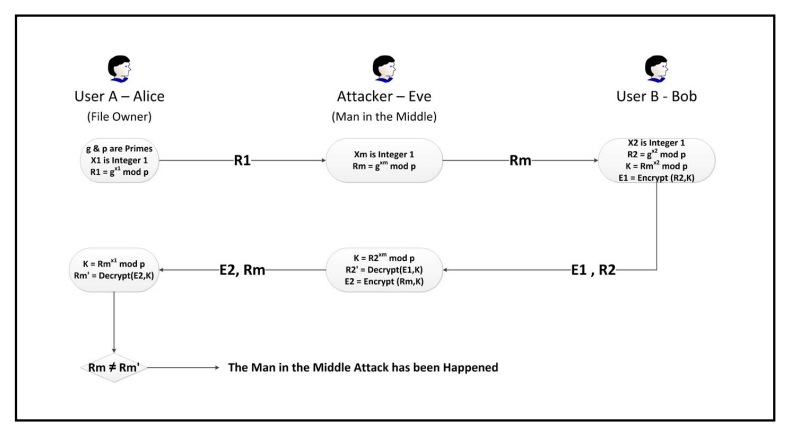
\includegraphics[width=160mm]{images/maninmiddle.png}{}
	\caption{ Man in the Middle Attack Prevention by Proposed Algorithm} %figure name
	\label{figmaninmiddle} % for referencing
\end{figure}

According to the figure, $R_{m}$ and $R^{'}_{m}$ are not same for
Alice because the keys between users and attackers are
different.\\
{$K_{Alice} = g^{x_{1}{x_{m}}}$ mod p}\\
{$K_{Bob} = g^{x_{2}{x_{m}}}$ mod p}\\
{$K_{Eve} = g^{x_{2}{x_{m}}}$ mod p}\\
It means $K_{Alice}$ $\neq$ $K_{Bob}$ = $K_{Eve}$  and because of that, the
Man in the Middle attack was noticed by Alice and the attack
was prevented.

\subsubsection{Cycle Attack }
Cycle Attack is an attack where the attacker encrypts the
cipher text alternately, until the original text appears. This
number of encrypting will decrypt any cipher text. In large key
RSA, this attack could not be practical even when a
generalisation of the attack allows the modulus to be factored
and most of the time it works faster. Moreover, in the
proposed model, the attacker will not have access to the public
key to re-encrypt the cipher text because the public key has
been encrypted by the secret key that was generated in
Modified Diffie-Hellman process.

\subsubsection{Brute Force Attack}
All possible combinations to guess the private key have
been tried by the attacker during Brute Force attack. In
original RSA, the probability of failure against this attack can
be decreased considerably by choosing exponents larger than
2048 bits but with the combination of the proposed model, this
algorithm has significant resistance towards brute force attack
even with 1024 bits exponents because of the encryption of
the public key before sending it.

\subsubsection{Timing Attack}
Timing attack is a side channel attack in which the attacker
determines private exponent by calculating the time by
exploiting the timing variation of the modular exponentiation
	[18]. Timing attack in original RSA might be prevented by
including a random delay to the exponentiation algorithm or
multiplying the cipher-text with a random number [19] while
the dual encryption (public key encryption by secret key and
the message encryption by RSA ) in the suggested model
will protect the transferred message from the timing attack and
it is not necessary to multiply the cipher-text.

\pagebreak
\subsection{CIA triad}
CIA triad is one of the most important models which is designed to guide policies
for information security within an organization.\\
CIA stands for :
Confidentiality,
Integrity,
Availability.\\
RSA with hashing, digital signature, and salting can provide confidentiality, integrity, and authenticity (CIA) for a message or data. \\
Here's how each component contributes to CIA protection:
\begin{itemize}
	\item Hashing: A secure hash function is used to produce a fixed-length hash value from the message or data.
	      This ensures the integrity of the message, as any changes to the original message will result in a different hash value.
	\item Salting: Salting is the process of adding random data to the input before hashing.
	      This makes it harder for an attacker to precompute hash values for commonly used inputs, such as passwords.
	      Salting increases the security of the hash value, as it makes it more difficult to guess the original input.
	\item RSA Encryption: The hash value is encrypted using the sender's private key, which creates a digital signature.
	      The recipient can verify the authenticity of the message by decrypting the digital signature using the sender's public key.
	      This ensures the authenticity of the message, as only the sender's private key can create the digital signature.
	\item Confidentiality: RSA encryption can also provide confidentiality by encrypting the original message with the recipient's public key.
	      This ensures that only the intended recipient can decrypt and read the message.\\

	      Overall, RSA with hashing, digital signature, and salting can provide CIA protection for messages or data, making it a useful tool in secure communication and data protection.
\end{itemize}






\pagebreak
\section{Software development model}
\subsection{Incremental Model}
\begin{figure}[H]
	\centering
	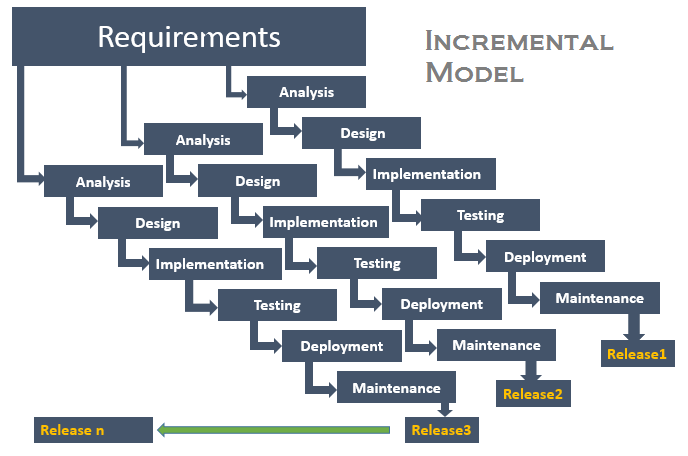
\includegraphics[width=160mm]{images/incremental model.png}{}
	\caption{Incremental Model Block Diagram} %figure name
	\label{figincremental} % for referencing
\end{figure}

\subsubsection{First Increment:}
First, the website was analyzed to know how it should look like.
Then, the designing of templates was done. After observing the design of the
templates, we started coding using react js, bootstrap, JavaScript.

\subsubsection{Second Increment:}
After analyzing the scenario of the project, the algorithms to be
implemented was analyzed. Using the algorithms, we started designing
the algorithms that is suitable for the project. Initiating the coding we
completed the algorithm implementation.
Finally, the algorithm was implemented.

\subsubsection{Third Increment:}
After the algorithm implementation backend designing and coding
was started. Using Django and Python the backend part
was completed and tested. Finally, backend was ready.

\subsubsection{Fourth Increment:}
Finally, after all the designing was completed, coding for the project was done. Later,
testing of the project was done.
At last, the final webapp was designed.
\pagebreak

\section{Block Diagram:}
\begin{figure}[H]
	\centering
	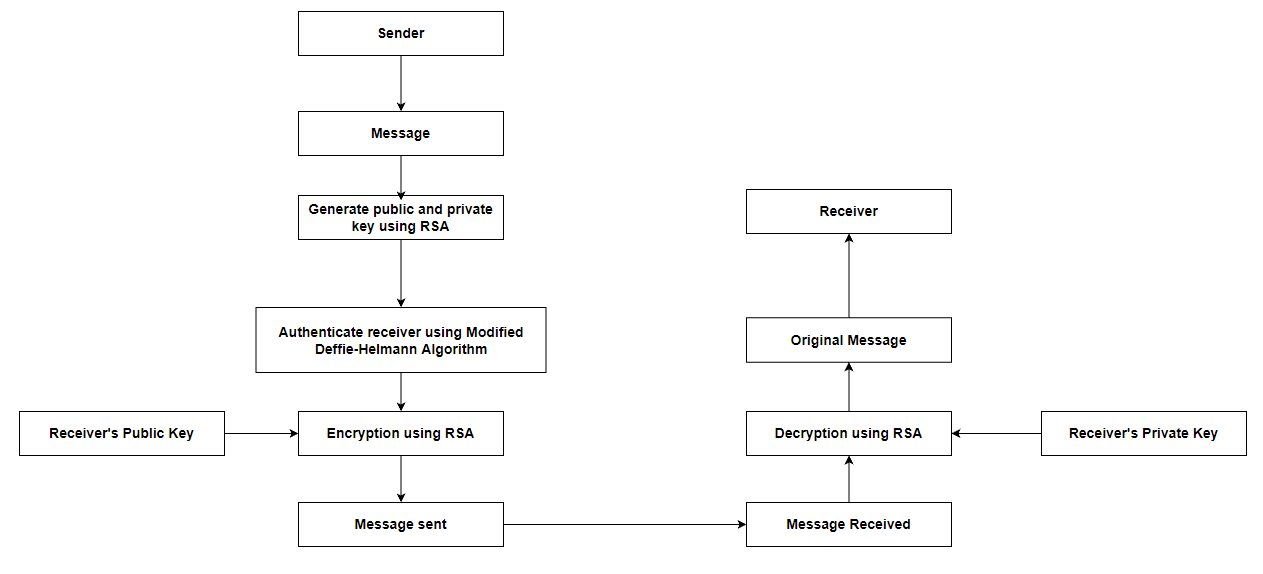
\includegraphics[width=170mm, height=160mm]{images/block diag.png}
	\caption{Block Diagram} %figure name
	\label{figblockdiagram} % for referencing
\end{figure}

\section{Use Case Diagram:}
\begin{figure}[H]
	\centering
	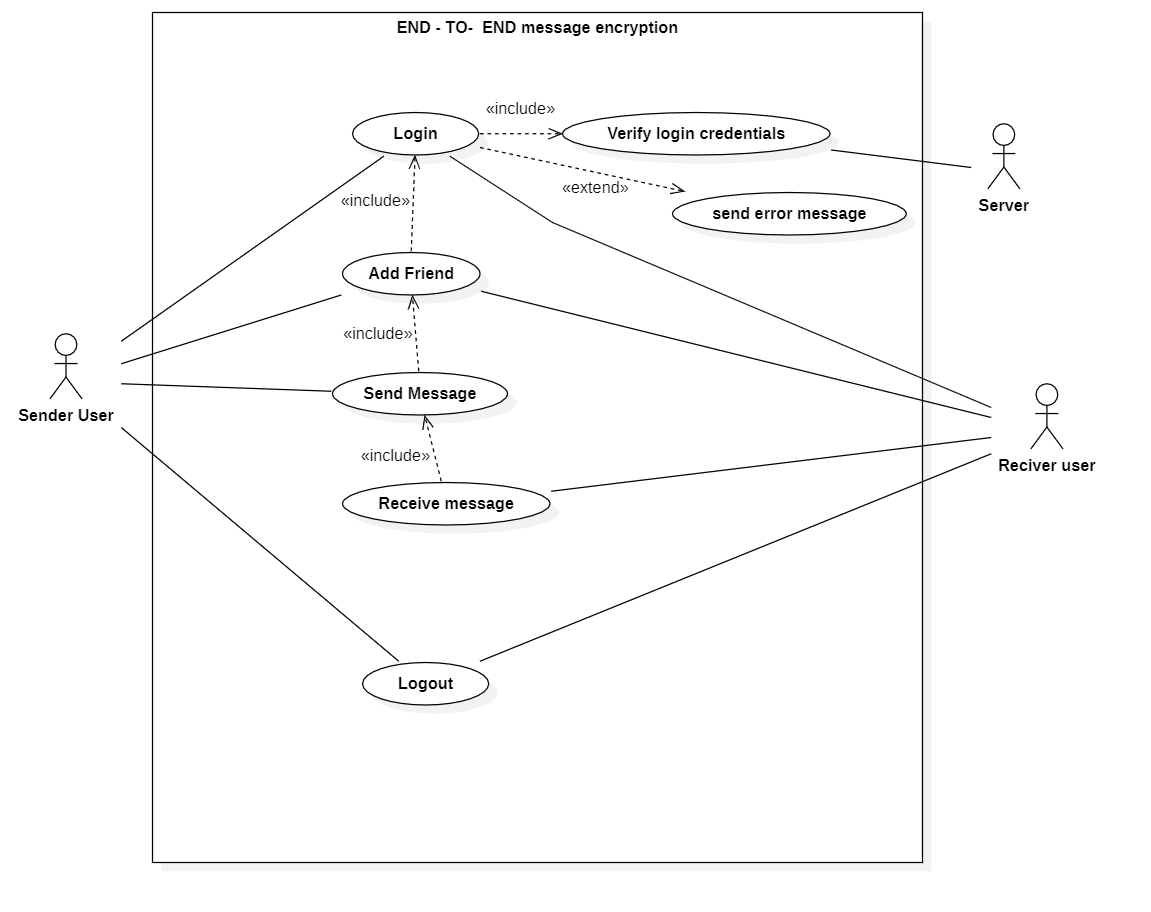
\includegraphics[width=180mm, height=180mm]{images/UseCaseDiagram1.png}
	\caption{Use Case Diagram} %figure name
	\label{figusecase} % for referencing
\end{figure}




\chapter{Epilogue}

\section{User Application}
Based on the observation of the system, we came to the following observation:
\vspace{-18pt}
\begin{itemize}
	\item The user application works well through all phase: signup and login, message sending and receiving. This make user experiene smooth.
	\item It is suitable for users who prioritize privacy in their communication. They allow users to have private conversations without fear of eavesdropping or surveillance from third parties.
\end{itemize}

\section{ Output:}
In the project hour, we researched on cryptography, chat app using cryptography, their advantages
disadvantages and probelms occured in chatapp etc. We developed chat app using react js, nodeJs, socket.io’
and RSA algorithm and Mongodb as database where we can send end to end encrypted text message between clients.

\begin{figure}[H]
	\centering
	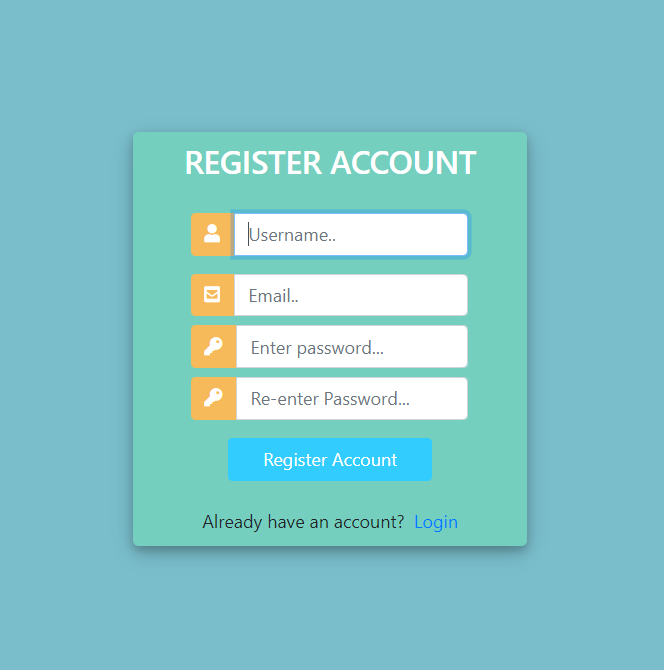
\includegraphics[width=160mm, height=180mm]{images/signup.png}
	\caption{Sign up interface} %figure name
	\label{figusecase} % for referencing
\end{figure}

\begin{figure}[H]
	\centering
	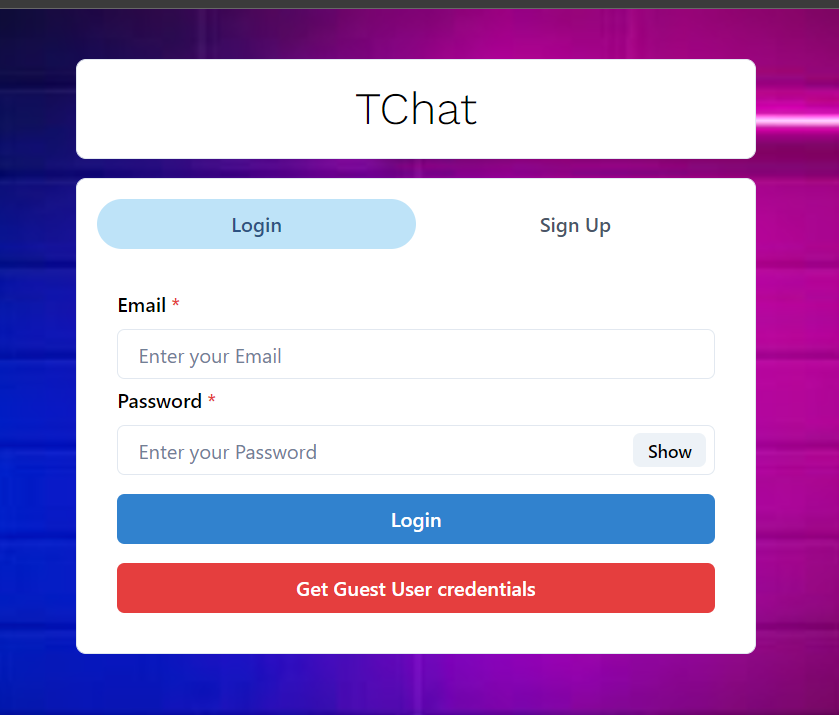
\includegraphics[width=160mm, height=180mm]{images/signin.png}
	\caption{Sign in interface} %figure name
	\label{figusecase} % for referencing
\end{figure}
\begin{figure}[H]
	\centering
	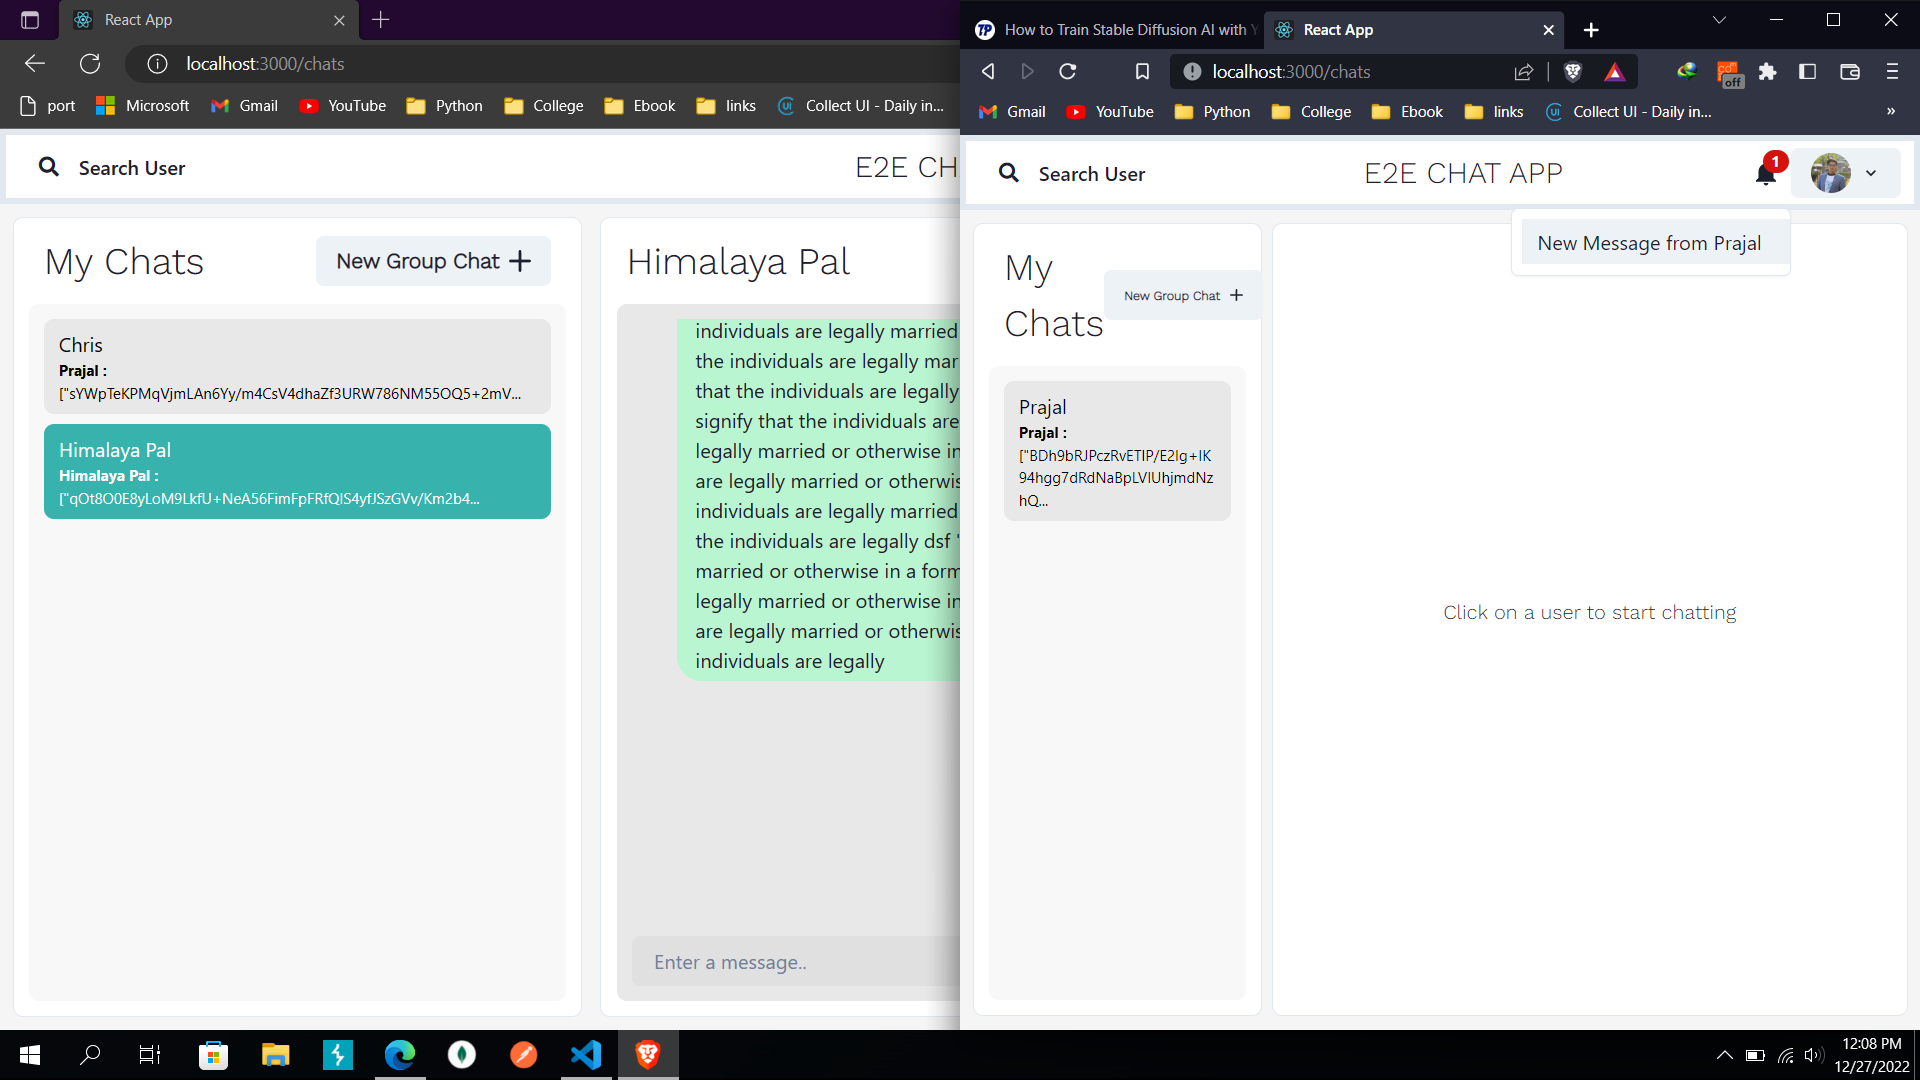
\includegraphics[width=160mm, height=160mm]{images/chat1.png}
	\caption{Chat interface} %figure name
	\label{figusecase} % for referencing
\end{figure}

%\section{Work on Progress:}
%%The ultimate goal of this project is to develop a working model of secure end to end chat web-app. This will include a working web client for user login and chat in real time using socket.io . We have finished creating login and signup system. Our program allows to search and add contacts; create a group chat. Our program also allows Users to send enrypted messages to each other.

%\section {Work Remaining:}
%We are still working on the backend and frontend  of the chat system. We are yet to integrate the DH algorithm to our current program. So far our program only allows encrypted chat between single users. We are yet to have encrypted group chat.


\section{Limitation}
The limitation of our system are listed below:
\vspace{-18pt}
\begin{itemize}
	\item Our chat application can send text message with 4000 character  at max. It is not available for audio, video, images messaging.
	\item The security measures taken can be complicated and require a lot of computing resources to implement, which can make the chat application bit slower to use.
	\item The system required the first internet connectivity for smooth operation.
\end{itemize}
\section{Future Enhancement}
This project can be further enhanced. Currently, we are able to send text message only but it can be developed to
send audio, video , images messaging chat app. We can add group chats options. As well as this project can be made more
secure with updates. Extra new trending features can be added in our system. We can also made this application compatible to all kind
of platforms and devices.

\section{Work Schedule}
Scheduling establishes the timelines, delivery and availability of project
resources whether they be personnel, inventory or capital. For this reason,
any project without a schedule is a project doomed to issue down the road.
The estimated time period of this project is 30 weeks. The work is divided into several
phases as shown in gantt chart.

\begin{figure}[H]
	\centering
	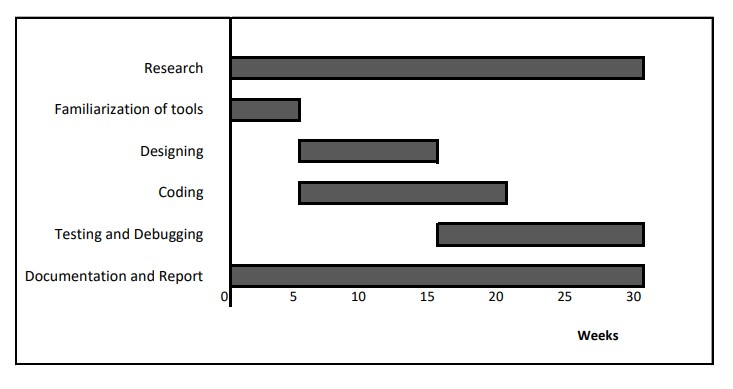
\includegraphics[width=160mm]{images/ganttchart.png.jpg}
	\caption{Gantt Chart} %figure name
	\label{figganttchart} % for referencing
\end{figure}

\section{Conclusion}
In this great era of technology data is more crucial than ever. The use of online messaging has resulted in more and more data to be shared between people from simple
messages to sensitive messages. As such need for some method to hide such confidential information is needed. Thus our project tries to do just that.





%Reference
\renewcommand\bibname{References} % Change heading to References
\bibliographystyle{IEEEtran} % to use IEEE Format for referencing
\addcontentsline{toc}{chapter}{References} % to add references in TOC
\bibliography{library} % specify the .bib file containing reference information 

%Comment this Chapter if you do not need to include Appendix.
%\chapter*{Appendix}
%\addcontentsline{toc}{chapter}{Appendix}
%Appendix Text Comes Here

\end{document}
